\documentclass{beamer}

\mode<presentation>
{
  \usetheme{default}     
  \usecolortheme{default} 
  \usefonttheme{default} 
  \setbeamertemplate{navigation symbols}{}
  \setbeamertemplate{caption}[numbered]
} 

\usepackage[english]{babel}
\usepackage[utf8x]{inputenc}
\usepackage[round]{natbib}
\usepackage{xcolor}
\usepackage{tikz}
\usepackage{caption}
\usetheme{CambridgeUS}
\usepackage{algorithm2e}


<<<<<<< HEAD:presentation/main.tex
\title[Changepoints]{Changepoint models of genomic data}
\author[]{Alan Chau \hspace{0.4cm}Ana Ignatieva\hspace{0.4cm} \\
James Thornton\hspace{0.4cm} Lorenzo Pacchiardi} % Your name
\institute{OxWaSP Module 2}
\date{02/11/18}

=======
>>>>>>> fb8c67cbb7dd605d170710875d55a1fa9fff83de:presentation/changepoints_ana.tex
\begin{document}

%{
%\usebackgroundtemplate{%
%\tikz\node[opacity=0.3]{\includegraphics[width=\paperwidth]{cover.pdf}};}
%\begin{frame}
%  \titlepage
%\end{frame}
%}

\title[Change Point Detection]{Change Point Detection in Genomic Data} % The short title appears at the bottom of every slide, the full title is only on the title page

\author[]{Alan Chau \hspace{0.4cm}Ana Ignatieva\hspace{0.4cm} \\
James Thornton\hspace{0.4cm} Lorenzo Pacchiardi} % Your name
\institute[Department of Statistics] % Your institution as it will appear on the bottom of every slide, may be shorthand to save space

\date{02/11/2018} % Date, can be changed to a custom date

\begin{frame}
\titlepage % Print the title page as the first slide
\end{frame}



%----------------------------------------------------------------------------------------
%	PRESENTATION SLIDES
%----------------------------------------------------------------------------------------

%------------------------------------------------
\section{Exact algorithm for detections} % Sections can be created in order to organize your presentation into discrete blocks, all sections and subsections are automatically printed in the table of contents as an overview of the talk
%------------------------------------------------


\begin{frame}
\frametitle{Long Chain DNA Sequences}
    \begin{figure}[h]
        \centering
        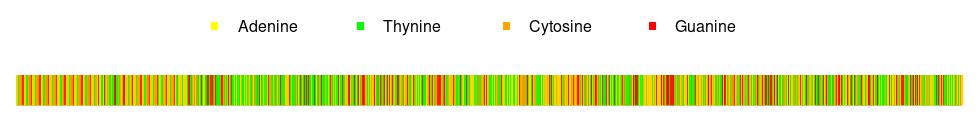
\includegraphics[scale=0.4]{5000_DNA.png}        
        \caption{Plot of a DNA with 5000 base pair}
        \label{fig:my_label}
    \end{figure}
\begin{itemize}
    \item Seemingly long and messy spectrum of A, T, C and G. Can you observe any structure?
\end{itemize}
\end{frame}

\begin{frame}
\frametitle{Long Chain DNA Sequences}
    \begin{figure}[h]
        \centering
        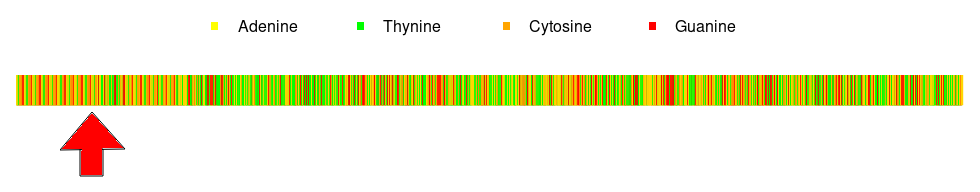
\includegraphics[scale=0.4]{5000_DNA_with_arrow.png}
        \caption{Plot of a DNA with 5000 base pair}
        \label{fig:my_label}
    \end{figure}
\begin{itemize}
    \item I found one after staring at the data for 2 days.
    \pause
    \item Is there a systematic way of doing this structure discovery?
    \pause
    \item In other words, can we detect change points systematically along this sequence?
\end{itemize}

\end{frame}

%------------------------------------------------

\begin{frame}
\frametitle{Talk Overview}
\begin{itemize}
\item Alan Chau - Exact algorithms for detections
\item Lorenzo Pacchiardi - Maximum Likelihood and approximate search methods
\item Ana Ignatieva - Hidden Markov Model
\item James Thornton - Bayesian Model and Grid-Merge
\end{itemize}
\end{frame}

%------------------------------------------------

\begin{frame}
\frametitle{Problem Statement}
\begin{itemize}
    \item Consider a sequence of data $\mathbf{y} = \{y_t\}_{t=1}^T$ where $y_t$ can be continuous, discrete or categorical. 
    \item Configure the set of possible change points as  $\mathcal{T}_{T} := \{\bm{\tau}: 0 = \tau_0 < \tau_1 < ... <\tau_K < \tau_{K+1} = T\}$
    \item We aim to minimise the following:
\begin{equation}
    V(\bm{\tau}, \mathbf{y}) = \min_{\bm{\tau} \in \mathcal{T}_{T}} \sum_{k = 0}^K \mathcal{C}(y_{\tau_k+1:\tau_{k+1}}) + \text{Pen}\{\bm{\tau}, \beta\}
\end{equation}
where $\mathcal{C}$ is some cost function measuring heterogeneity of the segment.
\end{itemize}
\end{frame}

\begin{frame}{Optimal Partitioning}
    \begin{itemize}
        \item One obvious choice is to pick the $L_0$ norm, $\beta K$ .
        \item Set $F(T)$ as $V(\bm{\tau}, \mathbf{y})$ restricted to the domain $\mathcal{T}_{T}$, we then realise:
        \begin{align}
        F(T) &= \min_{\bm{\tau} \in \mathcal{T}_T} \bigg\{
        \sum_{k = 0}^K\big[  \mathcal{C}(y_{\tau_k+1:\tau_{k+1}}) + \beta \big] \bigg\} \\
         &= \min_{t} \bigg\{ \sum_{k = 0}^{K-1}\big[  \mathcal{C}(y_{\tau_k+1:\tau_{k+1}}) + \beta \big] + \mathcal{C}(y_{t+1:T}) + \beta \bigg\} \\
         &= \min_{t} \{F(t) + \mathcal{C}(y_{t+1:T}) + \beta \}
\end{align}
    \item We can then use a dynamic program and start from $F(1)$ and obtain an exact solution in $\mathcal{O}(T^2)$
    \end{itemize}
\end{frame}

\begin{frame}{Pruned Exact Linear Time (PELT)}
    \begin{itemize}
        \item We get exactness but it is slow.  \pause
        \item We can use pruning to reduce complexity and achieve approximate linear run time. 
    \end{itemize}
\pause
\begin{theorem}
We assume there exits a constant K such that for all $t < s < T$,
$$\mathcal{C}(y_{t+1:s}) + \mathcal{C}(y_{s+1:T}) + K \leq \mathcal{C}(y_{t+1:T})$$
\noindent Then if 
$$F(t) + \mathcal{C}(y_{t+1:s}) + K \geq F(s) $$
\noindent holds, at a future time $T > s$, $t$ can never be the optimal last change point prior to $T$.
\end{theorem} 
\end{frame}

\begin{frame}{Pruned Exact Linear Time (PELT)}
    \begin{theorem}
We assume there exits a constant K such that for all $t < s < T$,
$$\mathcal{C}(y_{t+1:s}) + \mathcal{C}(y_{s+1:T}) + K \leq \mathcal{C}(y_{t+1:T})$$
\noindent Then if 
$$F(t) + \mathcal{C}(y_{t+1:s}) + K \geq F(s) $$
\noindent holds, at a future time $T > s$, $t$ can never be the optimal last change point prior to $T$.
\end{theorem} 
\begin{itemize}
    \item Intuitively speaking, if the condition is met, then s is always a better changepoint than t, thus we don't have to consider that anymore in future steps.
\end{itemize}
\end{frame}

\begin{frame}{Pruned Exact Linear Time}
\begin{algorithm}[H]
\caption{PELT Algorithm}
\SetAlgoLined
\textbf{Initialise: }Let $T$ be the number of data, set $F(0) = -\beta$, $cp(0) = NULL$ and $R_1 = \{0\}$ \\
\textbf{Iterate:} For $\tau^* = 1,...,T$
\begin{enumerate}
    \item Compute $F(\tau^*) = \min_{\tau \in R_{\tau^*}}[F(\tau) + \mathcal{C}(y_{\tau+1}:\tau^*) + \beta]$ 
    \item Let $\tau' = \arg\min_{\tau \in R_{\tau^*}}[F(\tau) + \mathcal{C}(y_{\tau+1:\tau^*}) + \beta ]$
    \item set $cp(\tau^*) = [cp(\tau'), \tau']$
    \item set $R_{\tau^* + 1} = \{\tau \in R_{\tau^*} \cap {\tau^*}: F(\tau) + \mathcal{C}(y_{\tau+1:\tau^*}) + K \leq F(\tau^*)\}$
\end{enumerate}
\textbf{Output: } A vector of change points in $cp(T)$
\end{algorithm}    
\end{frame}

\begin{frame}{Application}
    \begin{figure}
        \centering
        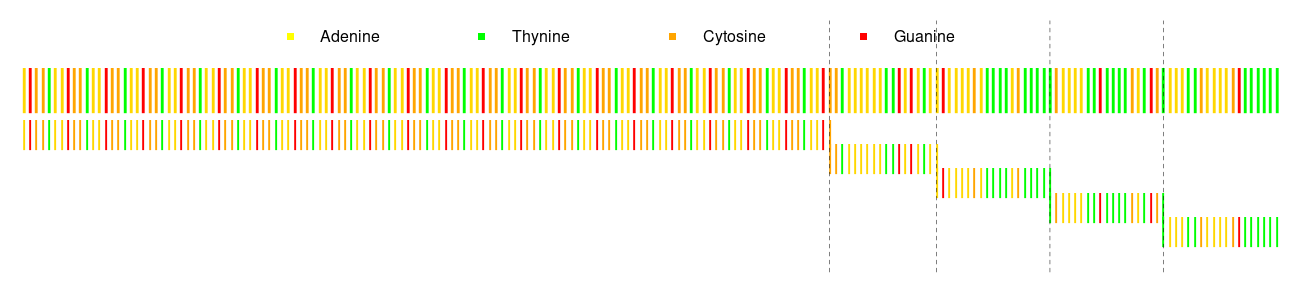
\includegraphics[scale=0.30]{DNA_seg.png}
        \caption{PELT applied to a sequence of DNA with length 200}
        \label{fig:my_label}
    \end{figure}
\end{frame}

\begin{frame}{Application}
    \begin{figure}
        \centering
        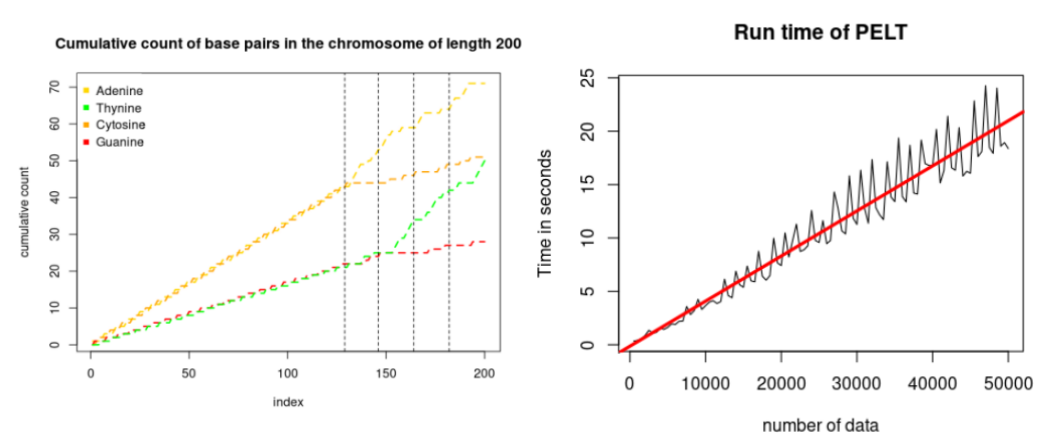
\includegraphics[scale=0.4]{runtime.png}
        \caption{(left) PELT applied to the first 200 DNA sequence. (right) Run time analysis on PELT}
        \label{fig:my_label}
    \end{figure}
\end{frame}

\begin{frame}{Problem with large sequences}
    \begin{figure}
        \centering
        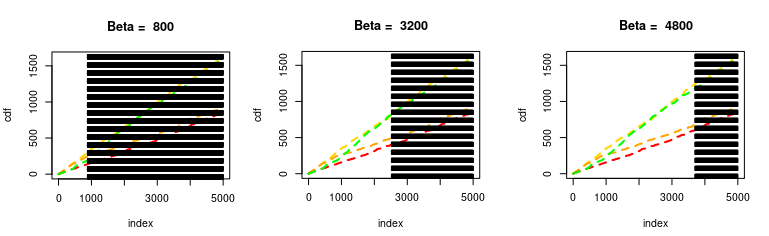
\includegraphics[scale=0.5]{PELT_limi.png}
        \caption{Limitation on the PELT method with large sequence}
        \label{fig:my_label}
    \end{figure}
\end{frame}

\begin{frame}{Pruned Exact Linear Time with Modified $L_0$ penalty}
\item To tackle this concentration of change points, we introduce a modified penalty for the PELT algorithm to control the spread,
\begin{equation}
    \label{modl0}
    \text{Pen}_{mL_0}(\bm{\tau}, \beta) = 3K\beta\log(T) + \beta\log(\beta)\sum_{k = 0}^K \log(\frac{\tau_{k+1} - \tau_{k}}{T})
\end{equation}

This can be easily incorporate to PELT by setting:
\begin{align}
    &\mathcal{C'}(y_{a+1:b}) \leftarrow \mathcal{C}(y_{a+1:b}) + \beta\log(\beta)\log\bigg({\frac{b-a}{T}}\bigg) & \beta' \leftarrow 3\beta\log(T)
\end{align}

\end{frame}

\begin{frame}{Results}
    \begin{figure}
        \centering
        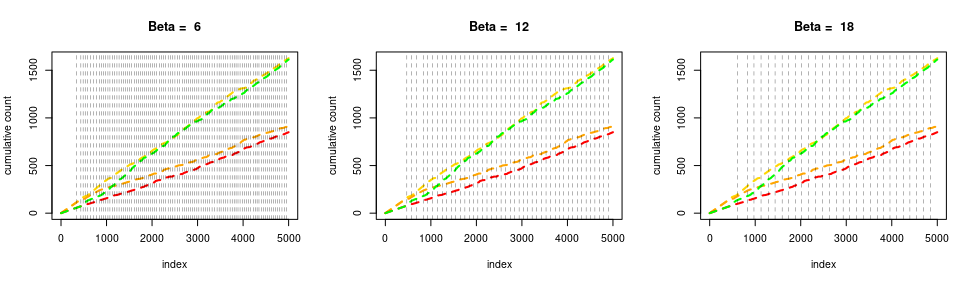
\includegraphics[scale=0.43]{PELTBIC_3.png}
        \caption{More evenly spread change points}
        \label{fig:my_label}
    \end{figure}
\end{frame}



%=============================================================================
% LORENZO
%=============================================================================

\section{MLE and approximate method for detection}

\begin{frame}{MLE of transition matrix}

Consider a standard Markov Chain. MLE for the transition probability:

\begin{equation*}\label{Eq:MLE}
\hat{p}_{ij} = \frac{n_{ij}}{\sum_{j=1}^m n_{ij}} = \frac{n_{ij}}{n_i} \longrightarrow p_{ij}
\end{equation*}

$n_{ij}$: number of observed transitions $ i\rightarrow j $
\end{frame}


\begin{frame}{MLE of transition matrix}
If the inferred segment is actually the composition of two MCs with different transition probabilities, we get: 

\begin{equation*}\label{}
	\hat{p}_{ij}  \longrightarrow \frac{N_0 p_i^0 p_{ij}^0 + N_1 p_i^1 p_{ij}^1}{N_0 p_i^0 + N_1 p_i^1}, \quad N_0,\ N_1 \rightarrow \infty
\end{equation*}

	\begin{figure}[h]
	\centering
	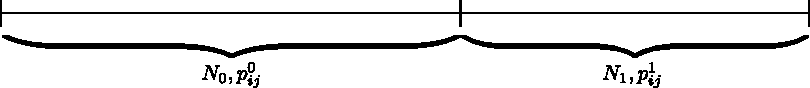
\includegraphics[width=1\linewidth]{MC.pdf}
	\vspace{-15pt}
%	\caption{}
%	\label{}
\end{figure}
\pause
 $\hat{p}_{ij} \rightarrow p_{ij}^0 \iff N_1/N_0 \rightarrow 0$.
\alert{This is usually not guaranteed in change point detection algorithms.}

\end{frame}


\begin{frame}{Markov model of genome segmentation \citep{thakur2007markov}}


\begin{itemize}

\item Recursive binary segmentation procedure. 

\item Maximizes Jensen Shannon divergence between the two subsequences $ S_1,\ S_2 $: $D_{JS}(S_1, S_2) = H(S) - \pi_1 H(S_1) - \pi_2 H(S_2) $

\item Each segmentation is accepted if it satisfies the BIC criterion $ \Delta \mathcal{C}_{BIC}<0 \iff 2ND_{JS}(S_1, S_2) > 16 \ln N $

\end{itemize}

\begin{figure}[h]
	\centering
	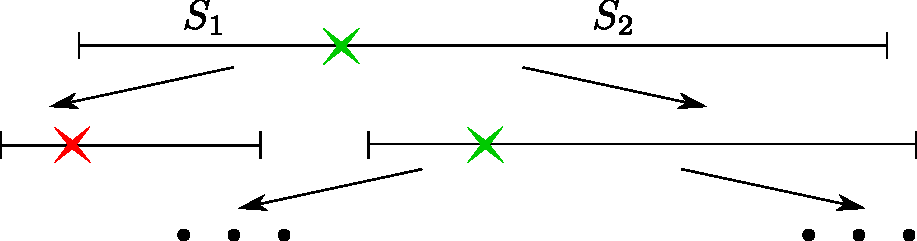
\includegraphics[width=1\linewidth]{binary_segmentation_alg.pdf}
%	\vspace{-15pt}
	%	\caption{}
	%	\label{}
\end{figure}

\end{frame}

\begin{frame}{Experiment on the genomic data}


%Validity of the algorithm is assessed on synthetic data.


\begin{itemize}

\item Time complexity $ \mathcal{O}(N \log_2 K) $, $ K $: number of change points.

\item Algorithm was run on the first 5 million nucleotides.
Segments for the first $ 1500 $ are reported in picture. 

\end{itemize}
	\begin{figure}[h!]
	\centering
	\begin{minipage}{.5\textwidth}
		\centering
		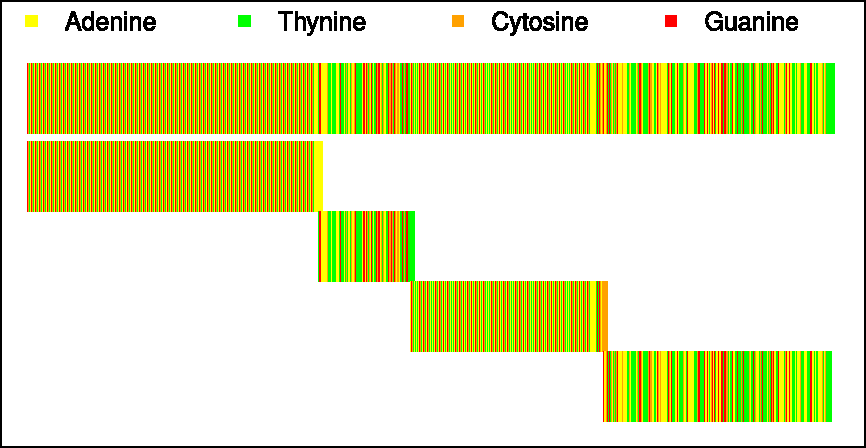
\includegraphics[width=1\linewidth]{DNA_segments.pdf}
		%			\caption{$dt=0.1$}
		%			\label{fig:prob1_6_2}
	\end{minipage}~
	\begin{minipage}{0.5\textwidth}
		\vspace{13pt}
		\centering
		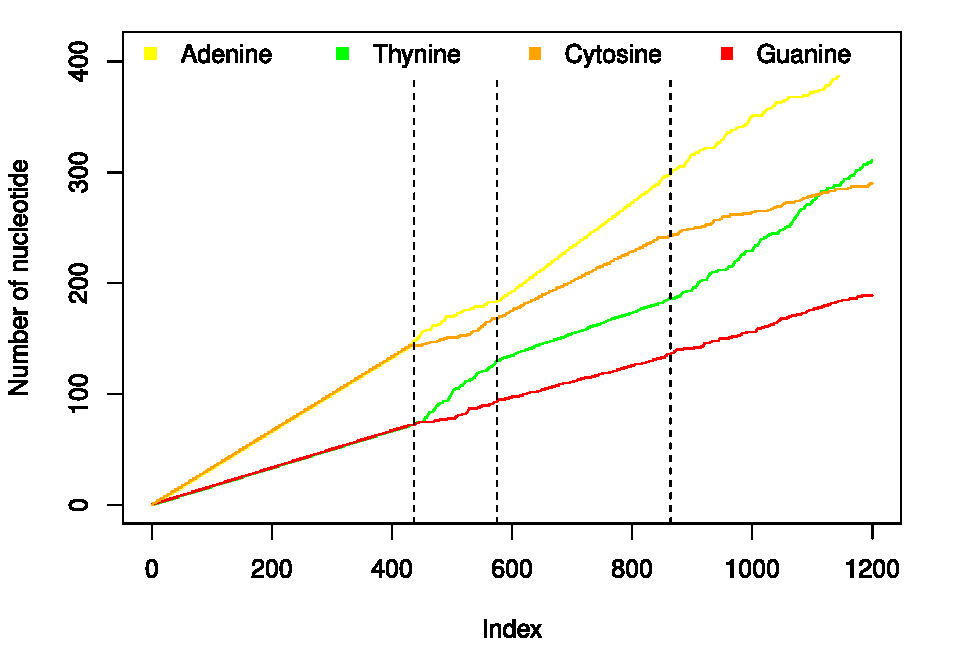
\includegraphics[width=1.0\linewidth]{DNA_segments_count_2.pdf}
		%			\caption{$dt =0.2$}
		%			\label{fig:prob1_6_1}
	\end{minipage}
\end{figure}

	
\end{frame}



%=============================================================================
% ANA
%=============================================================================


\section{Hidden Markov Models}

\subsection{HMMs}


\begin{frame}{HMM}
\begin{figure}
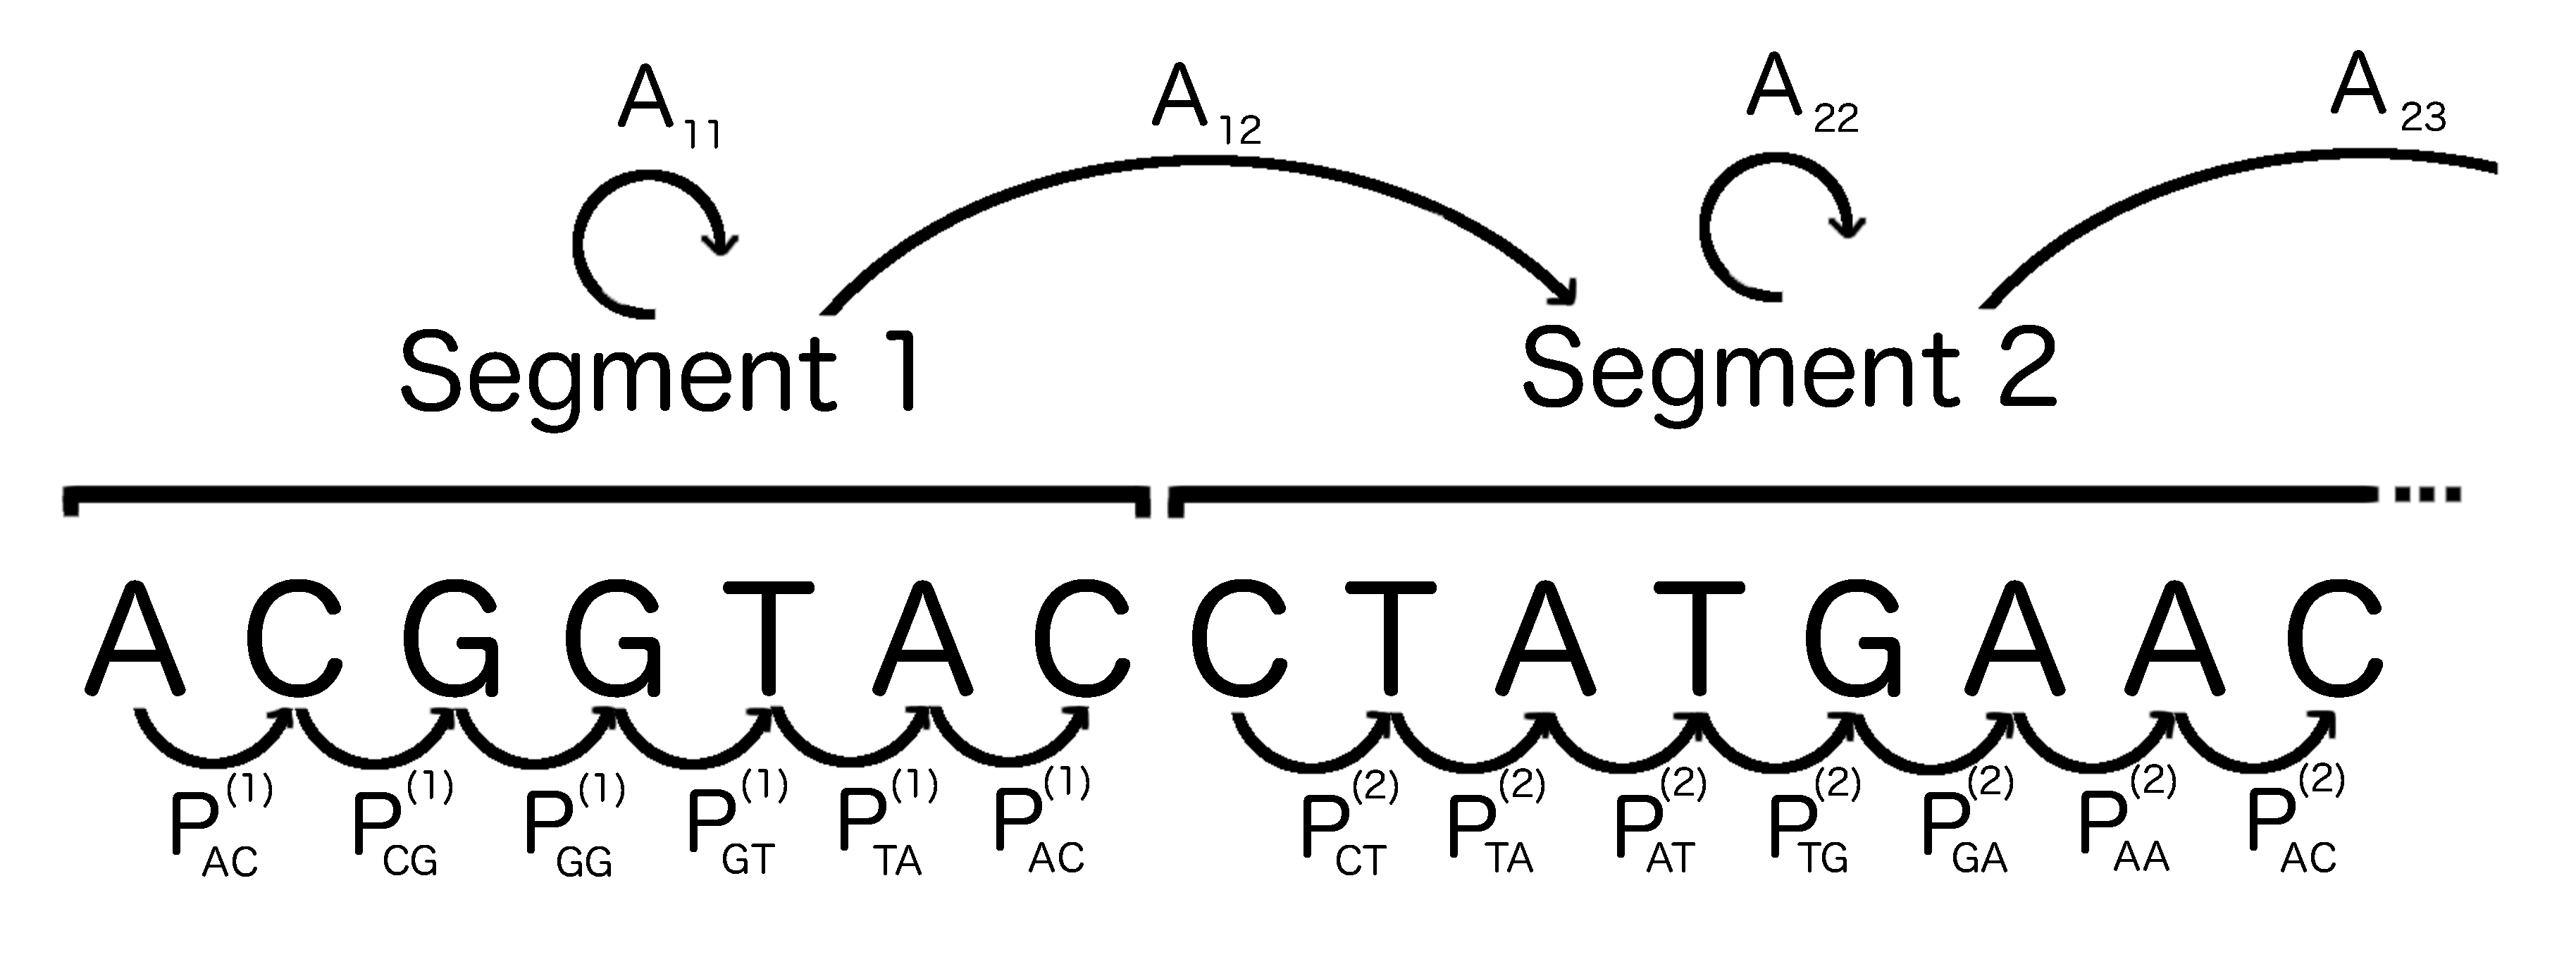
\includegraphics[width=\textwidth]{fig1.pdf}
\end{figure}
\begin{itemize}
\item $K$ hidden states, transition matrix $A$
\item Emissions $y_1, \hdots, y_T$, transitions $P_{ij}^{(s)}$
\item Changepoints = hidden state transitions
\item Used for genome data \citep{churchill, yeast}
\end{itemize}
\end{frame}


\begin{frame}{Hidden state transitions}
For changepoints want structure of $A$:
\[
\begingroup
\renewcommand*{\arraystretch}{2}
A = \left( {\begin{array}{ccccc}
1-\lambda_1 	& \lambda_1 	& 0 			& \hdots 				& 0\\
0 			& 1-\lambda_2 	& \lambda_2 	& \hdots				& 0\\
\vdots 		&			& \ddots		& \ddots					& 0\\
0 			& \hdots	 	& 0		 	& 1-\lambda_{K-1} 		& \lambda_{K-1} \\
0			& \hdots		& 0			& 0					& 1 \\
\end{array}} \right)
\endgroup
\]
\begin{itemize}
\item Small probability of transitioning to next state
\item Can't revisit previous states
\item Can't jump ahead
\end{itemize}
\end{frame}


\begin{frame}{Parameter fitting}
Baum-Welch \citep{durbin}:
\begin{itemize}
\item Version of E-M
\item Need to incorporate Markov dependency of emissions
\item Iteratively compute $\mathbb{P}(S_t | y_1, \hdots, y_T)$
\item Expected number of times $(i j)$ appears in state $s$ 
\item[ ] $\implies$ update $P_{ij}^{(s)}$
\item Expected number of state transitions $i \rightarrow j$
\item[ ] $\implies$ update $A_{ij}$
\end{itemize}
\vspace{20pt}
Decode the HMM:
\begin{itemize}
\item Viterbi: get most likely path through states
\item Posterior $\mathbb{P}(S_t | y_1, \hdots, y_T)$
\end{itemize}
\end{frame}


\begin{frame}{Simulated data}
\begin{figure}
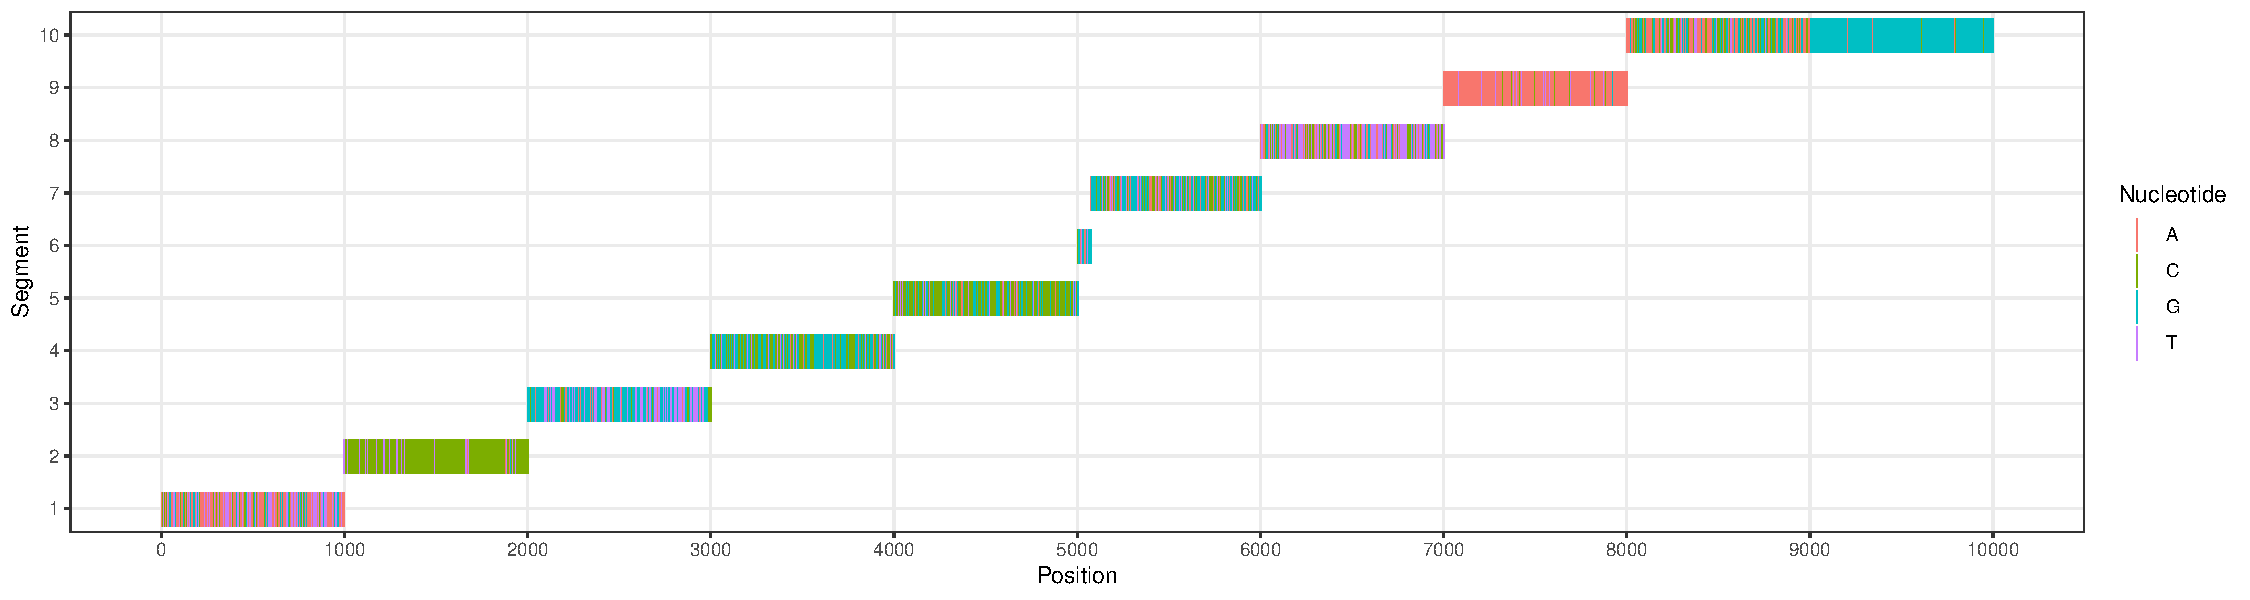
\includegraphics[width=\textwidth]{fig2.pdf}
\end{figure}
\begin{itemize}
\item Actual changepoints at every 1,000
\item Almost!
\end{itemize}
\end{frame}

\begin{frame}{Real data}
\begin{figure}
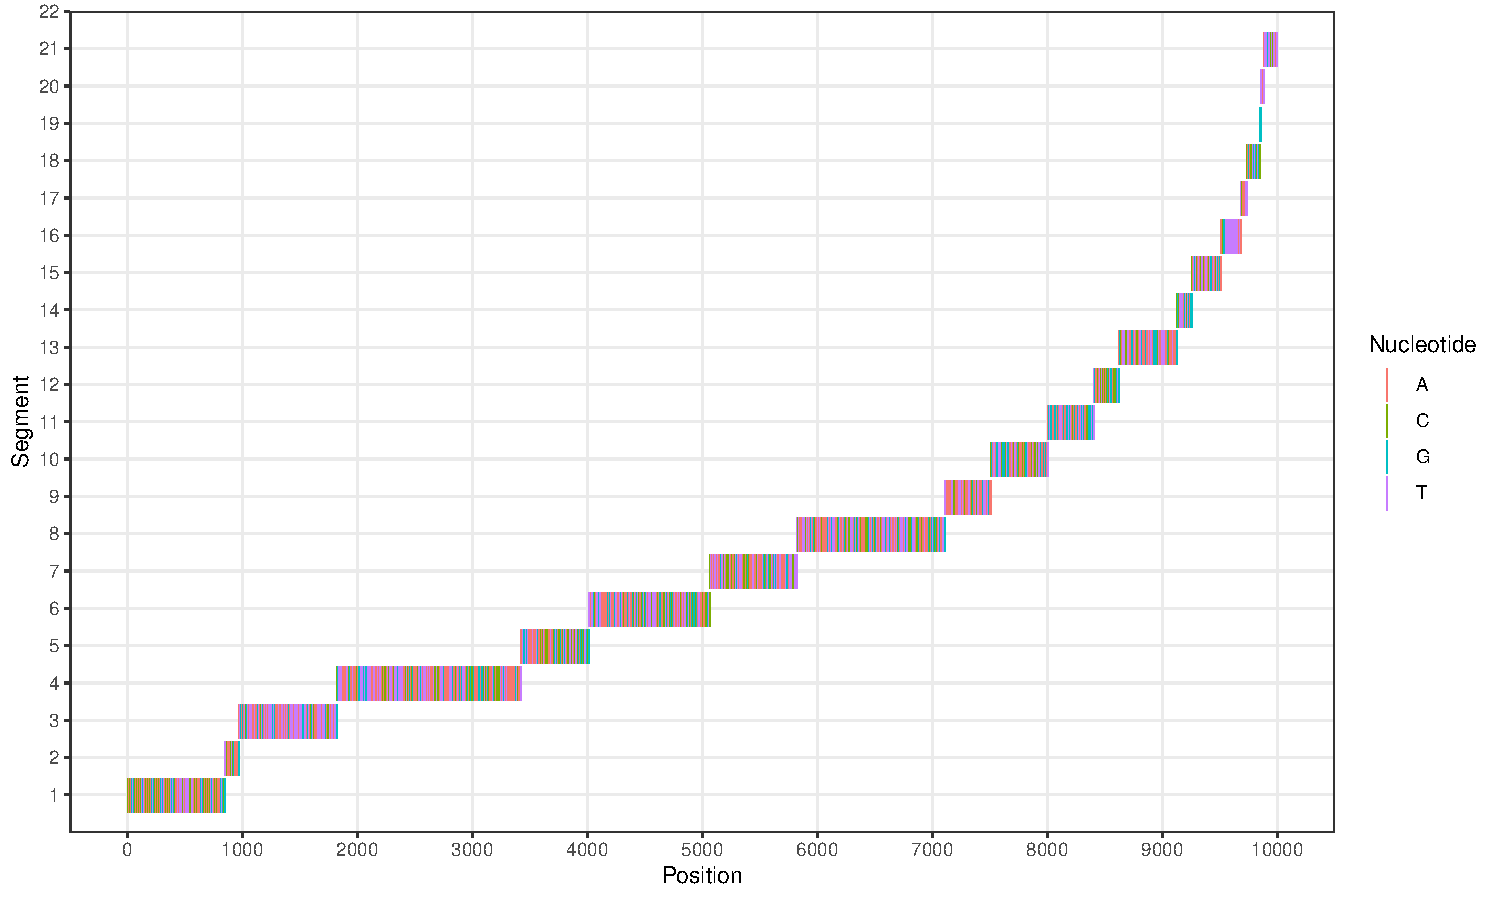
\includegraphics[width=0.9\textwidth]{fig3.pdf}
\end{figure}
\begin{itemize}
\item Initial guess for max number of changepoints = 50
\item HMM finds 22
\end{itemize}
\end{frame}

\begin{frame}{Conclusions}
\begin{itemize}
\item Flexible:
\begin{itemize}
\item number of changepoints
\item incorporate information into structure of $A$
\end{itemize}
\item General class of models
\item Relatively slow
\end{itemize}
\end{frame}

%=============================================================================
% JAMES
%=============================================================================

\section{Bayesian HMM and Grid-Merge}
\begin{frame}{Bayesian Change Point Detection}

\begin{minipage}{.4\linewidth} 
\centerline{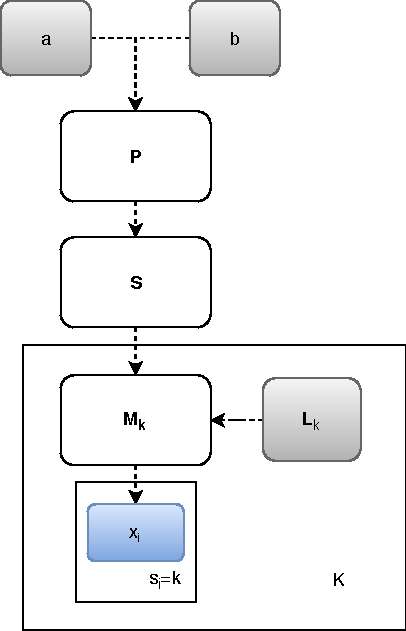
\includegraphics[scale=0.6]{Bayesian_Change_Point_Detection.pdf}}
\end{minipage}
\begin{minipage}{.5\linewidth}
\fontsize{8}{7.2}\selectfont
Generative Model:
\begin{itemize}
	\item $P           \sim BetaDiag(a,b)$
	\item $\mathcal{S} \sim MarkovChain(P) \text{ where } s_1=1$
	\item $M_k | \mathcal{S}      \sim  DirMat(\boldsymbol{\lambda}) \text{ } \forall k \in [1:K]$
	\item $x^k_{1:n_k}|\mathcal{S},M_k \sim MarkovChain(M_k)$
\end{itemize}
\vspace{1cm}

Implementation:
\begin{itemize}
	\item Conjugate
	\item MCMC
	\begin{itemize}
		\fontsize{8}{7.2}\selectfont
		\item Blocked Gibbs Sampling
		\item Simulated annealing
	\end{itemize}
\end{itemize}

\end{minipage}
\end{frame}

\begin{frame}{Grid-Merge Heuristic}

Split chain index $\rightarrow$ Merge on distance between MLE transition matrices $\rightarrow \ldots$ \\
\vspace{.5cm}
\centerline{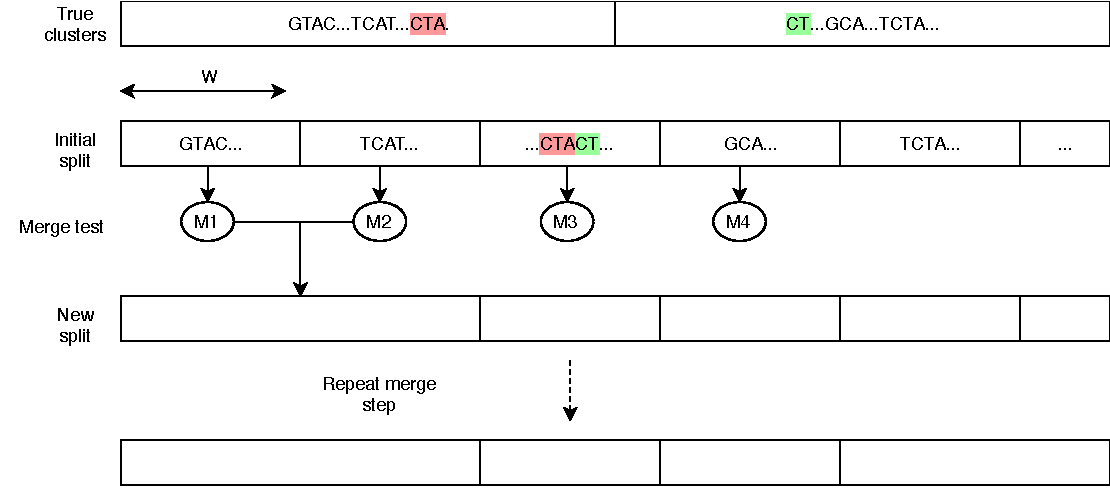
\includegraphics[scale=0.5]{Grid_Merge.pdf}}

\begin{itemize}
	\item Applicable for large data-sets
	\item Intuitive interpretation
	\item Approximation error
\end{itemize}

\end{frame}

\begin{frame}{Results on Simulated Data}
\centerline{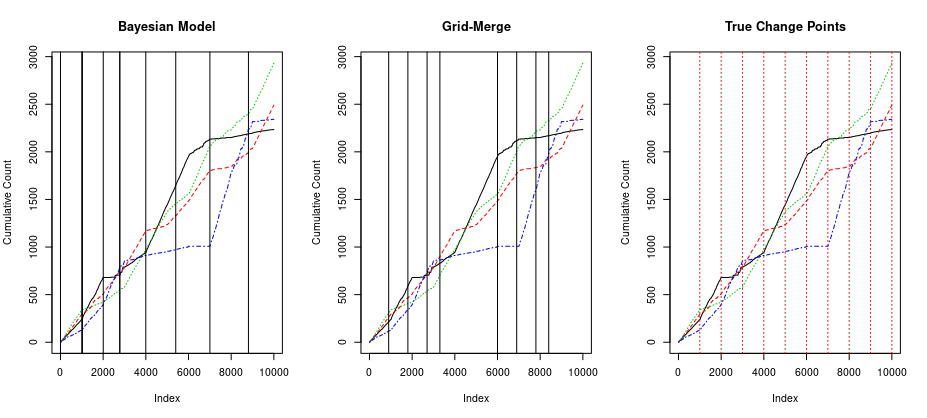
\includegraphics[scale=0.5]{comp_hor.png}}
\end{frame}

%=============================================================================

\begin{frame}
\bibliographystyle{plainnat}
\bibliography{bibliography}
\end{frame}


\end{document}



















